\chapter{Appendix A}

\section{Preliminary definitions}

\begin{definition}\label{Def:Sylvester matrix}
The Sylvester matrix \(\text{Syl}(-,-)\) of two polynomials 
\begin{equation*}
A = a_n x^n + a_{n-1}x^{n-1} + \dots a_0, \quad
B = b_m x^m + b_{m-1}x^{m-1} + \dots b_0
\end{equation*}
of degree \(n\) and \(m\) respectively is the \(n+m\)-matrix given by
\begin{equation*}
{Syl}(A,B) = 
\begin{bmatrix}
     a_0 &0 &\dots &0 &b_0 &0 &\dots &0 \\
     a_1 &a_0 &\dots &0 &b_1 &b_0 &\dots &0 \\
     a_2 &a_1 &\ddots &\vdots &b_2 &b_1 &\dots &\vdots \\
     \vdots &\vdots &\ddots &a_0 &\vdots &\vdots &\ddots &b_0\\
     a_n & a_{n-1} &\dots &\vdots &b_m & b_{m-1} &\dots &\vdots \\
     0 & a_n &\ddots &\vdots &0 & b_m &\ddots &\vdots\\
     \vdots &\vdots &\ddots &a_{n-1} &\vdots &\vdots &\ddots &b_{m-1}\\
     0 &0 &\dots &a_n &0 &0 &\dots &b_m
\end{bmatrix}.
\end{equation*}
%
By description, this matrix consists of the coefficients of the two polynomials placed vertically from the start, and then shifting the entries along the diagonal of the matrix. It is easier to see how this works by looking at example \ref{Ex:R-point}. Sometimes in other literature, the Sylvester matrix may be defined as the transpose of how we define it here. 
%
\end{definition}
%
\begin{definition}\label{Def:Presheaf}
%
Let X be a topological space, and \(\mathcal{C}\) some category. A presheaf on X is a functor F with values in \(\mathcal{C}\), such that for every open set \(U\) in X, there is an object \(F(U)\) in \(\mathcal{C}\). Also we demand some compatibility, which is done by having:
For every pair of open subsets of X, say (U,V) there is a morphism \(r_{U,V}:F(U)\longrightarrow F(V)\) in \(\mathcal{C}\). We demand that the morphism r corresponding to any open set \(U \subset X\) is the identity morphism on \(F(U)\), i.e. \(id_U = r_{U,U}:F(U)\longrightarrow F(U)\). Also, for any triple of subsets of X, say \(W\subset V\subset U\), the diagram
\begin{center}
    \begin{tikzcd}
F(U) \arrow[rd, "{r_{U,V}}"'] \arrow[rr, "{r_{U,W}}"] &  & F(W) \\
 & F(V) \arrow[ru, "{r_{V,W}}"'] & 
\end{tikzcd} commutes.
%
\end{center}
%
\end{definition}
%
\begin{definition}\label{Def:Sheaf}
%
A sheaf is a presheaf with some extra restrictions on how the attached structures behave in the intersections of open subsets of our space X. In particular we force two extra axioms. \\
%
\textbf{Identity axiom}. Let \(\{U_i\}_i\) be an open cover of \(U\), and let \(f,g\in F(U)\). If \(r_{U,U_i}(f) = r_{U, U_i}(g)\) for all \(i\), then \(f = g\). \\
%
\textbf{Gluability axiom}. Let \(\{U_i\}_i\) be an open cover of \(U\), and \(\forall i\), let \(f_i \in F(U_i)\) s.t. \(r_{U_i, U_i\cap U_j}(f_i) = r_{U_j, U_i \cap U_j}\) for all \(i\) and \(j\).  Then there exists \(f\in F(U) \) s.t. \(\forall i, r_{U, U_i}(f) = f_i \).
%
\end{definition}
%
\begin{definition}\label{Def:Local ring}
A ring R is said to be a local ring if it satisfies one of the following equivalent properties:
\begin{enumerate}
    \item R has a unique left maximal ideal
    \item R has a unique right maximal ideal
    \item \(1 \neq 0\) and the sum of any two non units is again a non unit. 
    \item \(1 \neq 0\) and for any element \(x\in R\), either \(x\) or \(1-x\) is a unit. 
\end{enumerate}
\end{definition}

%\begin{definition}\label{Def:Stalks of a sheaf}
%Define stalks of sheaf
%\end{definition}

\begin{definition}\label{Def:Affine scheme}
An affine scheme is a locally ringed topological space, i.e. Its a topological space together with a sheaf of rings, s.t. all of the stalks of the sheaf are local rings. 
\end{definition}

\begin{definition}\label{Def:Spectrum of a ring}
Let R be a ring. As a set, Spec(R) is defined to be the set of prime ideals in R. We then augment is with a topology called the Zariski topology. It is defined by letting the closed sets of Spec(R) be defined by the vanishing sets V(S) of all subsets S of R. The vanishing set is defined by
%
\begin{equation*}
    V(S) := \{[P] \in \text{Spec}(R) | S \subset P \}.
\end{equation*}
%
For this to be a topology, we must also allow any other set forced to be closed by these sets to be closed. The Zariski topology has a nice basis by the distinguished open sets. If \(f\in R\), the distinguished open set of \(f\) is defined by
%
\begin{equation*}
    D(f) := \{[P] \in \text{Spec}(R) | f \notin P \}.
\end{equation*}
%
It is the "non-vanishing"- set of \(f\). \\
To make the final step from a topological space to a scheme, we must define a sheaf on Spec(R). We call this sheaf the structure sheaf on Spec(R), denoted \(\mathcal{O}_{\text{Spec}(R)}\), and we define it by letting \(\mathcal{O}_{\text{Spec}(R)}(D(f)) := F(D(f)) = R_f\), i.e. the localization of R at the powers of \(f\). It can be checked that this forms a sheaf on Spec(R). \\
%
\begin{remark}
It can be shown that every affine scheme is isomorphic to Spec(A) for some ring A, and hence some authors use the definition of an affine scheme to be a ringed space isomorphic to Spec(A) for some A. 
\end{remark}
%
\end{definition}

\begin{definition}\label{Def:Scheme}
A scheme is a locally ringed space which admits a covering of open subsets \(\{U_i\}\) such that each \(U_i\) is an affine scheme. This means that schemes are topological spaces which locally look like affine schemes. Globally we glue the affine schemes together with the Zariski topology. By the previous remark, we can also define a scheme to be a topological space that is locally isomorphic to Spec(A) for some ring A. 
\end{definition}

\section{Example of \(\mathbb{A}_{k}^1\)}


\begin{example}\label{Ex:Complex affine line}
The complex affine line is a scheme constructed in the following way
\begin{equation*}
	\mathbb{A}^1(\mathbb{C}) = \text{Spec}(\mathbb{C}[x]) . 
\end{equation*}
Since this example is just to gain intuition on how to think about simple schemes, we describe this just as a set. \\
Lets find the prime ideals of \(\mathbb{C}[x]\). Since \(\mathbb{C}[x]\)is an integral domain, we know \((0)\) is prime. We also know that \((x-a)\) is prime for \(a \in \mathbb{C}\) since they are maximal ideals. This we know because
\begin{center}
\begin{tikzcd}
0 \arrow[r] & (x-a) \arrow[r] & {\mathbb{C}[x]} \arrow[r, "f\to f(a)"] & \mathbb{C} \arrow[r] & 0
\end{tikzcd}
\end{center}
is exact, proving that the quotient is a field, thus maximal, thus prime. \\
We need to show that there is no other prime ideals, so assume we have a prime ideal \((P)\neq (0)\). Suppose \(0 \neq f(x)\in (P)\) has smallest degree. We know \(f(x)\) is not constant, since any prime ideal cant contain \(1\). If then \(f(x)\) is not linear, by the fundamental theorem of algebra, we can factor \(f(x)=f_1(x)f_2(x)\) where they both have nonzero positive degree. By the primality of \((P)\), either \(f_1(x)\in (P)\) or \(f_2(x)\in (P)\), but this contradicts the minimality of the degree of \(f\), and thus \(f\) is linear, i.e. \(f(x)=x-a\). 

This proves we have a linear element in \((P)\), and our claim is now that \((P)=(x-a)\). Suppose we have an element \(g(x)\in (P)\). Since \(\mathbb{C}[x]\) has a division algorithm, we get that \(g(x)=h(x)(x-a)+c\), where \(c\in \mathbb{C}\). We can thus express a constant in terms of elements in \((P)\), so if \(c\) is nonzero this contradicts there being no constant elements in \((P)\) by earlier in the proof. Hence \(c=0\) and we have \(g(x)=h(x)(x-a)\) for every \(g(x)\in (P)\), which proves \((P)\) is generated by \(x-a\). 

Now we have found all the points in the spectrum. This now makes the complex affine line a little more intuitive. We can naturally associate each of the prime ideals \(x-a\) to the element \(a\in \mathbb{C}\), which makes a long list of all the complex numbers. Now you may ask: "Where is \((0)\)?". It is not a stupid question, since it is nowhere and everywhere at the same time. Remember that \((0)\subset (P)\) for every prime ideal \((P)\), but it is also a proper point in \(\text{Spec}(\mathbb{C}[x])\).  If we visualize \(\mathbb{A}^1(\mathbb{C})\) as a long list of numbers from left to right, we can think of \((0)\) as the line connecting them all. 

We will not go deep into why we think of \(\mathbb{A}^1(\mathbb{C})\) as a line, and not a plane, but it stems from a purely algebraic notion of dimension. This version of dimension is called Krull dimension. Readers who find algebraic dimensionality interesting, want more examples of spectrums or to build a more complete intuition on schemes, are referred to \cite[chapter 3, 4, 5 and 11]{Vakil}. 
\newline

\begin{center}



\begin{figure}
    \centering

\tikzset{every picture/.style={line width=0.75pt}}

%set default line width to 0.75pt        

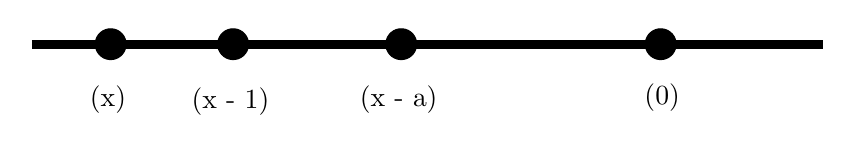
\begin{tikzpicture}[x=0.75pt,y=0.75pt,yscale=-1,xscale=1]
%uncomment if require: \path (0,300); %set diagram left start at 0, and has height of 300


%Straight Lines [id:da22332223838056997] 
\draw [color={rgb, 255:red, 0; green, 0; blue, 0 }  ,draw opacity=1 ][fill={rgb, 255:red, 0; green, 0; blue, 0 }  ,fill opacity=1 ][line width=3]    (99.3,100.47) -- (480.3,100.47) ;


%Shape: Circle [id:dp6643237363432828] 
\draw  [fill={rgb, 255:red, 0; green, 0; blue, 0 }  ,fill opacity=1 ] (129.89,99.88) .. controls (130.16,95.8) and (133.69,92.7) .. (137.78,92.98) .. controls (141.87,93.25) and (144.96,96.78) .. (144.69,100.87) .. controls (144.42,104.96) and (140.88,108.05) .. (136.79,107.78) .. controls (132.71,107.5) and (129.61,103.97) .. (129.89,99.88) -- cycle ;
%Shape: Circle [id:dp3426760131435296] 
\draw  [fill={rgb, 255:red, 0; green, 0; blue, 0 }  ,fill opacity=1 ] (188.89,99.88) .. controls (189.16,95.8) and (192.69,92.7) .. (196.78,92.98) .. controls (200.87,93.25) and (203.96,96.78) .. (203.69,100.87) .. controls (203.42,104.96) and (199.88,108.05) .. (195.79,107.78) .. controls (191.71,107.5) and (188.61,103.97) .. (188.89,99.88) -- cycle ;
%Shape: Circle [id:dp29970333704367036] 
\draw  [fill={rgb, 255:red, 0; green, 0; blue, 0 }  ,fill opacity=1 ] (269.89,99.88) .. controls (270.16,95.8) and (273.69,92.7) .. (277.78,92.98) .. controls (281.87,93.25) and (284.96,96.78) .. (284.69,100.87) .. controls (284.42,104.96) and (280.88,108.05) .. (276.79,107.78) .. controls (272.71,107.5) and (269.61,103.97) .. (269.89,99.88) -- cycle ;
%Shape: Circle [id:dp5094461474575767] 
\draw  [fill={rgb, 255:red, 0; green, 0; blue, 0 }  ,fill opacity=1 ] (394.89,99.88) .. controls (395.16,95.8) and (398.69,92.7) .. (402.78,92.98) .. controls (406.87,93.25) and (409.96,96.78) .. (409.69,100.87) .. controls (409.42,104.96) and (405.88,108.05) .. (401.79,107.78) .. controls (397.71,107.5) and (394.61,103.97) .. (394.89,99.88) -- cycle ;

% Text Node
\draw (136,127) node  [align=left] {(x)};
% Text Node
\draw (195,128) node  [align=left] {(x - 1)};
% Text Node
\draw (276,127) node  [align=left] {(x - a)};
% Text Node
\draw (403,126) node  [align=left] {(0)};


\end{tikzpicture}

    \caption{Visualization of \(\mathbb{A}_{\mathbb{C}}^1\).}
    \label{fig:Affine line}
\end{figure}
\end{center}
\end{example}


